\documentclass[11pt]{exam}
\newcommand{\myname}{Ling Song, Hosein Hadipour} %Write your name in here
\newcommand{\myhwtype}{Homework}
\newcommand{\myhwnum}{1} %Homework set number
\newcommand{\myclass}{Cryptanalysis 2021}
\newcommand{\mylecture}{}
\newcommand{\mysection}{}

% Prefix for numedquestion's
\newcommand{\questiontype}{Question}

% Use this if your "written" questions are all under one section
% For example, if the homework handout has Section 5: Written Questions
% and all questions are 5.1, 5.2, 5.3, etc. set this to 5
% Use for 0 no prefix. Redefine as needed per-question.
\newcommand{\writtensection}{0}

\usepackage{amsmath, amsfonts, amsthm, amssymb}  % Some math symbols
\usepackage{enumerate}
\usepackage{enumitem}
\usepackage{graphicx}
\usepackage{hyperref}
\usepackage[all]{xy}
\usepackage{wrapfig}
\usepackage{fancyvrb}
\usepackage[T1]{fontenc}
\usepackage{listings}

\usepackage{centernot}
\usepackage{mathtools}
\DeclarePairedDelimiter{\ceil}{\lceil}{\rceil}
\DeclarePairedDelimiter{\floor}{\lfloor}{\rfloor}
\DeclarePairedDelimiter{\card}{\vert}{\vert}


\setlength{\parindent}{0pt}
\setlength{\parskip}{5pt plus 1pt}
\pagestyle{empty}

\def\indented#1{\list{}{}\item[]}
\let\indented=\endlist

\newcounter{questionCounter}
\newcounter{partCounter}[questionCounter]

\newenvironment{namedquestion}[1][\arabic{questionCounter}]{%
    \addtocounter{questionCounter}{1}%
    \setcounter{partCounter}{0}%
    \vspace{.2in}%
        \noindent{\bf #1}%
    \vspace{0.3em} \hrule \vspace{.1in}%
}{}

\newenvironment{numedquestion}[0]{%
	\stepcounter{questionCounter}%
    \vspace{.2in}%
        \ifx\writtensection\undefined
        \noindent{\bf \questiontype \; \arabic{questionCounter}. }%
        \else
          \if\writtensection0
          \noindent{\bf \questiontype \; \arabic{questionCounter}. }%
          \else
          \noindent{\bf \questiontype \; \writtensection.\arabic{questionCounter} }%
        \fi
    \vspace{0.3em} \hrule \vspace{.1in}%
}{}

\newenvironment{alphaparts}[0]{%
  \begin{enumerate}[label=\textbf{(\alph*)}]
}{\end{enumerate}}

\newenvironment{arabicparts}[0]{%
  \begin{enumerate}[label=\textbf{\arabic{questionCounter}.\arabic*})]
}{\end{enumerate}}

\newenvironment{questionpart}[0]{%
  \item
}{}

\newcommand{\answerbox}[1]{
\begin{framed}
\vspace{#1}
\end{framed}}

\pagestyle{head}

\headrule
\header{\textbf{\myclass\ \mylecture\mysection}}%
{\textbf{\myname}}%
{\textbf{\myhwtype\ \myhwnum}}

\begin{document}
\thispagestyle{plain}
\begin{center}
  {\Large \myclass{} \myhwtype{} \myhwnum} \\
  \myname{}\\
  \today
\end{center}


%Here you can enter answers to homework questions
\begin{numedquestion}
	This concerns using memory in favor of speed in implementing the encryption algorithms. Let $S$ be the AES S-box. Let $MC$ be the mix-column, i.e., it takes as input a column consisting of 4 bytes and outputs such a column. Note that $MC$ is linear, i.e., we have for any two columns $C_{1}, C_{2}$ that:
	\begin{equation*}
	MC(C_{1} \oplus C_{2}) = MC(C_{1})\oplus MC(C_{2}). 
	\end{equation*}
	
	Define a function $T_{0}$ as follows: it takes as input a byte $b$, and the output $T_{0}(b)$ is a 4-byte column computed as follows: you first form a column $C(b)$ by placing $S(b)$ in the top byte and all-0 bytes in the lower three positions. Then set $T_{0}(b) = MC(C(b))$. We also define functions $T_{1}, T_{2}, T_{3}$. They are similar to $T_{0}$, except that when we form $C(b)$, we place $S(b)$ in the second, third and fourth entry from the top respectively, and put in 0's elsewhere. 
	
	Now consider the state of AES encryption algorithm at the start of some round. Name the bytes in this state $a_{ij}$ as in ? and let $R$ be the state after we have done \texttt{SubBytes}, \texttt{ShiftRow} and \texttt{MixColumn}. So $R$ is a 4 by 4 matrix of bytes. 
	
	Show that the first column of $R$ is
	\begin{equation*}
	T_{0}(a_{00})\oplus T_{1}(a_{11}) \oplus T_{2}(a_{22}) \oplus T_{3}(a_{33}).
	\end{equation*}
	Give similar expressions for the other 3 columns of $R$. 
	
	Sketch how this result can be used to implement AES based only on table look-up and XOR, instead of explicitly computing the operations. How much memory would you need for this?  
	
	\begin{figure}[ht!]
		\begin{center}
			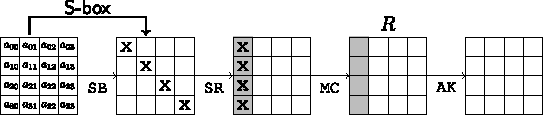
\includegraphics[scale=1.5]{./Figures/aes_round_function.pdf}
		\end{center}\caption{A Round of AES} \label{fig:aes_round_function}
	\end{figure}
	
\end{numedquestion}

\begin{numedquestion}
	Consider the following structure where ENC and DEC represent the encryption and decryption via the \texttt{DES} algorithm with 56-bit key respectively. Note that, the first and last encryption blocks use the same 56-bit key $k_{1}$, whereas the middle one utilizes $k_{2}$ which is not necessarily the same as $k_{1}$. Does it provide the $112$-bit security level? If not so, provide a cryptographic attack with time complexity of strictly less than $2^{112}$ \texttt{DES} encryptions. Please explain what model is your attack classified in (known-plaintext, chosen-plaintext, $\ldots$). Besides, the amount of \textbf{time} and \textbf{memory} in your attack should be specified in detail.
	
	\textit{A known plaintext attack has more points in comparison to a chosen plaintext attack.}
	\begin{figure}[ht!]
		\begin{center}
			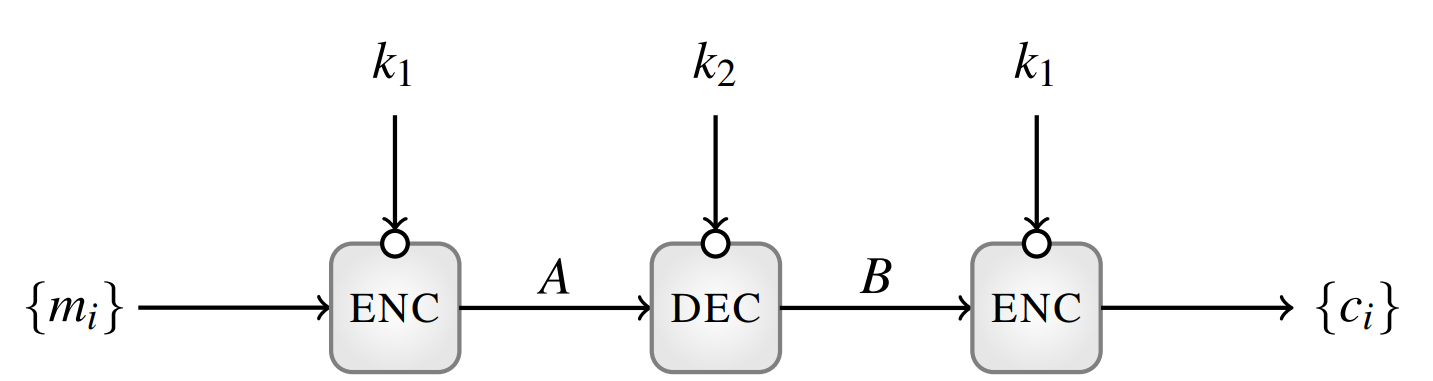
\includegraphics[scale=0.5]{./Figures/two_key_triple_encryption.PNG}
		\end{center}\caption{Two-Key Triple Encryption} \label{fig:two_key_three_encryptions}
	\end{figure}
\end{numedquestion}

\begin{numedquestion}
\textit{It is usually much easier to find matching objects than it is to find a particular object!}

\begin{alphaparts}
\item What is the probability that someone has the same birthday as you? 
\item What is the probability that at least two people share the same birthday?
\item In a group of 23 strangers, what is the probability that at least two of them have the same birthday? How about if there are 40 strangers?
\item In a group of 200 strangers, what is the probability that one of them has the same birthday as your birthday?  
\end{alphaparts}
\end{numedquestion}

\begin{numedquestion}
An urn contains $N$ balls, of which $n$ are red and $N - n$ are blue. Bob randomly selects a ball from the urn, replaces it in the urn, randomly selects a second ball, replaces it, and so on. He does this until he has looked at a total of $m$ balls. 
\begin{alphaparts}
\item Prove that Bob selects at least one red ball with the following probability: 
\begin{equation*}
\Pr(\text{at least one red}) = 1 - \left(1 - \frac{n}{N}\right)^{m}.
\end{equation*}
\item Prove that a lower bound for the above probability is:
\begin{equation*}
\Pr(\text{at least one red}) \geq 1 - e^{-\frac{m\cdot n}{N}}.
\end{equation*}
\item Prove that if $N$ is large and if $m$ and $n$ are not too much larger than $\sqrt{N}$ (e.g., $m, n\leq 10\sqrt{N}$), then the two sides of the above inequality are almost the same.
	\item Bob has a box that contains $N$ numbers. he chooses $n$ distinct numbers from the box and puts them in a list. he then makes a second list by choosing $m$ (not necessarily distinct) numbers from the box. Prove that if $n$ and $m$ are each slightly larger than $\sqrt{N}$, then it is very likely ($\Pr \geq 0.5$) that the two lists contain a common elements. 
	
\textit{Hint: In the previous question, assume that all balls are blue at first. Then, Bob selects $n$ balls one at a time to construct the first list. Next, he repaints those $n$ balls with the red paint and return them to the box. The second list is constructed by drawing $m$ balls out of the urn one after another, noting its number and color, and then replacing it.}
\item 
Assume that $H:\{0, 1\}^{\*}\rightarrow \{0, 1\}^{n}$ is a hash function, where $n\in \mathbb{N}$. Prove that, regardless of the internal structure of $H$, a collision can be found with high probability in $\mathcal{O}(2^{\frac{n}{2}})$ steps, where $\mathcal{O}(2^{\frac{n}{2}})$ words of memory are used. 
\end{alphaparts}
\end{numedquestion}

% if you do not solve some of the questions use this command to increment counter
% \setcounter{questionCounter}{4}
\begin{numedquestion}
Assume that $f$ is a function from $S = \{1, \ldots, N\}$ to itself where $N\in \mathbb{N}$. In addition, $f$ is easy to evaluate but hard to invert. We are given a value $y\in S$ and are asked to find its preimage $x$ under $f$, i.e., $y = f(x)$.  Let $x_{1}^{0}, \ldots, x_{m}^{0}$ be some elements of $S$. Build the following array of chains: 
\begin{align*}
	&x_{1}^{0} \longrightarrow x_{1}^{1} = f(x_{1}^{0}) \longrightarrow & \cdots & \longrightarrow x_{1}^{t} = f(x_{1}^{t - 1}),\\
	&x_{2}^{0} \longrightarrow x_{2}^{1} = f(x_{1}^{0}) \longrightarrow & \cdots & \longrightarrow x_{1}^{t} = f(x_{2}^{t - 1}),\\
	&\cdots & \cdots & \\
	&x_{m}^{0} \longrightarrow x_{m}^{1} = f(x_{1}^{0}) \longrightarrow & \cdots & \longrightarrow x_{m}^{t} = f(x_{m}^{t - 1}),\\
\end{align*}
where $t\in \mathbb{N}$. 
	\begin{alphaparts}
		\item Given a $y\in S$, how would you check the existence of $x$ (such that $f(x) = y$) among the first $t$ columns of the above array if you are merely given the first and the last columns of the above array?
		\item Assuming that all elements inside the $0$'th through $t - 1$'st columns of the above array are different, compute the probability of appearing $x$ among the first $t$ columns.
		\item By the birthday paradox, prove that if we add new a new row to the above array, the additional row have likely no common point with the previous ones as long as $t\cdot mt \leq N$. Hence, choosing $m$ and $t$ such that $mt^{2} > N$ will not be a good choice. 
		\item If we choose $m$ and $t$ such that the relation $mt^{2} = N$ is satisfied, then a single array like above covers only a fraction $\frac{mt}{N} = \frac{1}{t}$ of $S$. On the other hand, constructing additional tables using the same strategy as above, increases the probability of reappearing the same points in different tables which causes us to waste a lot of space! So, what is your solution to cover the whole $S$? 
		\end{alphaparts}
\end{numedquestion}

\begin{numedquestion}
This concerns a trick that is very useful to find a cycle in a sequence of iterated function values. Let $S$ be any finite set, $f$ be any function from $S$ to itself, and $x_{0}$ be any element of $S$. For any $i > 0$, let $x_{i} = f(x_{i - 1})$. Let $\mu$ be the smallest index such that the value $x_{\mu}$ reappears infinitely often within the sequence of values $x_{i}$, and let $\lambda$ be the smallest positive integer such that $x_{\mu} = x_{\lambda + \mu}$.
\begin{figure}[ht!]
	\begin{center}
		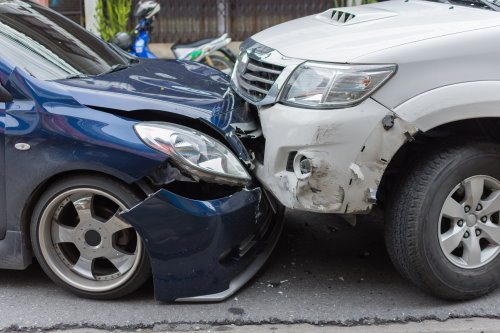
\includegraphics[scale=0.5]{./Figures/collision2.jpeg}
	\end{center}\caption{Collisions for Truncated \texttt{SHA3}} \label{fig:collisions}
\end{figure}
\begin{alphaparts}
\item 
Prove that $i = k\lambda \geq \mu$ for some $k$ if and only if $x_{i} = x_{2i}$. 
\item Based on the above fact, propose an algorithm to find $\mu$ and $\lambda$, given $f$ and $x_{0}$. 
\item Using the proposed algorithm in the previous part, find a 64-bit collision for $\texttt{SHA3-512}$. 
\end{alphaparts}
Hint: Study about the cycle detection algorithms in \url{https://en.wikipedia.org/wiki/Cycle_detection}.

To compute the $\texttt{SHA3-512}$ using the \texttt{Python} language you can use the following commands: 
\begin{lstlisting}[language=Python]
In [1]: import hashlib
In [2]: st = "Hello World!"
In [3]: digest = hashlib.sha3_512(st.encode())
In [4]: digest.hexdigest()
Out[4]: '32400b5e89822de254e8d5d94252c52bdcb27a3562ca593e980364d9848b8041
b98eabe16c1a6797484941d2376864a1b0e248b0f7af8b1555a778c336a5bf48'
\end{lstlisting}
\end{numedquestion}
\end{document}